\documentclass[12pt]{article}
\usepackage[paperwidth=28cm, paperheight=14cm, margin=0.7cm]{geometry}
\usepackage{xcolor}
\usepackage{tikz}
\usepackage{amsmath}
\usepackage[utf8]{inputenc}
\usepackage[T1]{fontenc}
\usetikzlibrary{arrows.meta, positioning, fit, backgrounds, calc}
\pagestyle{empty}

\definecolor{C0}{HTML}{2E86AB}
\definecolor{C1}{HTML}{A23B72}
\definecolor{C2}{HTML}{F18F01}
\definecolor{C3}{HTML}{1B998B}
\definecolor{C4}{HTML}{E84855}
\definecolor{Cbg}{HTML}{F4F7FA}
\pagecolor{Cbg}

\begin{document}
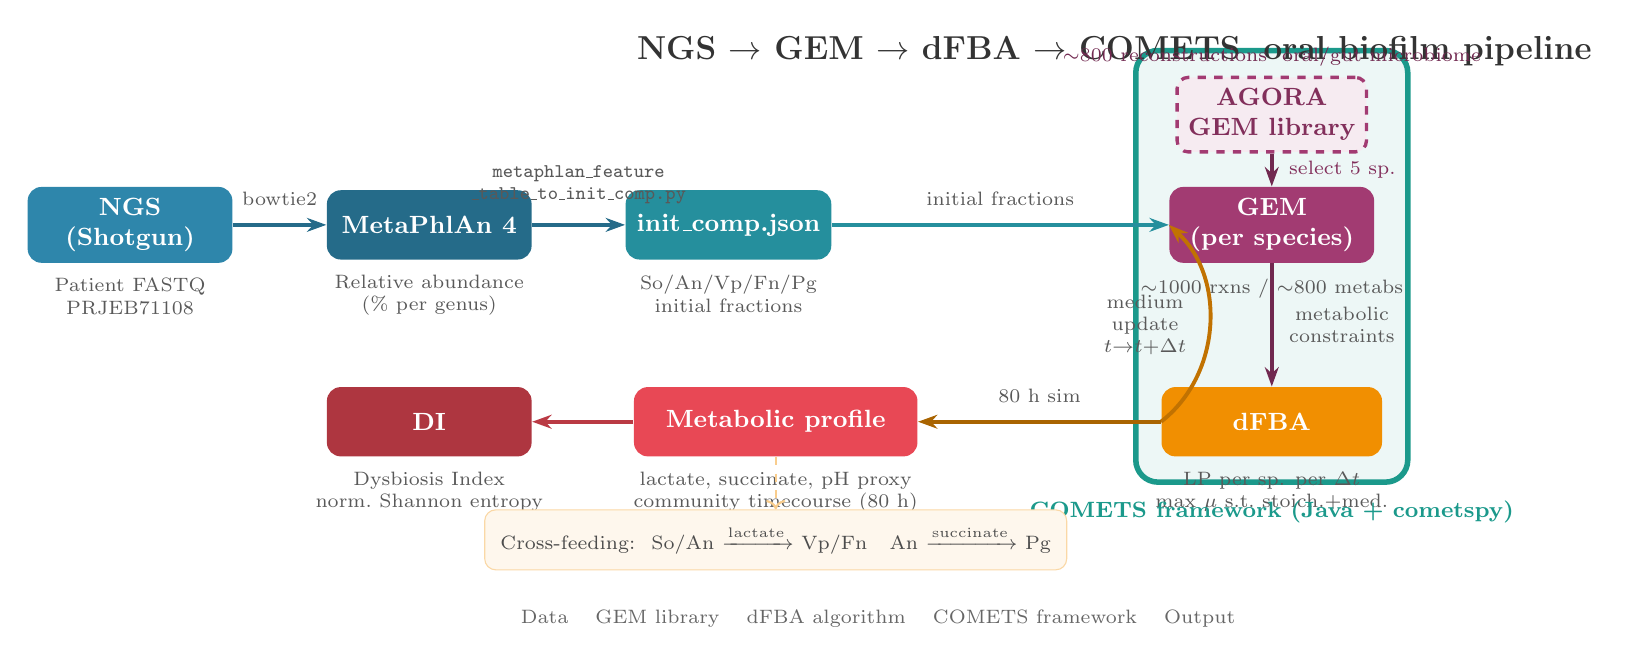
\begin{tikzpicture}[
    x=1cm, y=1cm,
    every node/.style={font=\small},
    box/.style={rounded corners=5pt, minimum width=2.6cm, minimum height=0.88cm,
                align=center, text=white, font=\small\bfseries, inner sep=4pt},
    arr/.style={-{Stealth[length=7pt,width=5pt]}, line width=1.4pt},
    lbl/.style={font=\scriptsize, align=center, text=black!65},
    lib/.style={rounded corners=4pt, minimum width=2.4cm, minimum height=0.78cm,
                align=center, draw, font=\small\bfseries, dashed,
                line width=1.2pt, inner sep=4pt},
]

% ─── Title ────────────────────────────────────────────────
\node[font=\large\bfseries, text=black!80] at (12.5, 12.2)
    {NGS $\to$ GEM $\to$ dFBA $\to$ COMETS\; oral biofilm pipeline};

% ─── Row 1 (y=10.0): data flow ────────────────────────────
\node[box, fill=C0]          (ngs)  at (0.0,  10.0) {NGS\\(Shotgun)};
\node[box, fill=C0!80!black] (meta) at (3.8,  10.0) {MetaPhlAn 4};
\node[box, fill=C0!55!C3]    (init) at (7.6,  10.0) {init\_comp.json};

\node[lbl, below=0.07cm of ngs]  {Patient FASTQ\\PRJEB71108};
\node[lbl, below=0.07cm of meta] {Relative abundance\\(\% per genus)};
\node[lbl, below=0.07cm of init] {So/An/Vp/Fn/Pg\\initial fractions};

\draw[arr, C0!80!black] (ngs.east)  -- (meta.west)
    node[midway, above=0.1cm, lbl]{bowtie2};
\draw[arr, C0!80!black] (meta.east) -- (init.west)
    node[midway, above=0.12cm, lbl]
        {\texttt{metaphlan\_feature}\\\texttt{\_table\_to\_init\_comp.py}};

% ─── AGORA (y=11.4) ───────────────────────────────────────
\node[lib, C1, fill=C1!10, text=C1!80!black]
    (agora) at (14.5, 11.4) {AGORA\\GEM library};
\node[lbl, above=0.0cm of agora, text=C1!70!black]
    {${\sim}800$ reconstructions\ \ oral/gut microbiome};

% ─── GEM (y=10.0) ─────────────────────────────────────────
\node[box, fill=C1] (gem) at (14.5, 10.0) {GEM\\(per species)};
\node[lbl, below=0.07cm of gem]
    {${\sim}1000$ rxns\ /\ ${\sim}800$ metabs};

\draw[arr, C1!70!black] (agora.south) -- (gem.north)
    node[midway, right=0.08cm, lbl, text=C1!80!black]{select 5 sp.};

% init_comp → GEM
\draw[arr, C0!55!C3] (init.east) -- (gem.west)
    node[midway, above=0.1cm, lbl]{initial fractions};

% ─── dFBA (y=7.5) ─────────────────────────────────────────
\node[box, fill=C2, minimum width=2.8cm]
    (dfba) at (14.5, 7.5) {dFBA};
\node[lbl, below=0.07cm of dfba]
    {LP per sp. per $\Delta t$\\ $\max\,\mu$\ s.t.\ stoich.$+$med.};

\draw[arr, C1!70!black] (gem.south) -- (dfba.north)
    node[midway, right=0.08cm, lbl]{metabolic\\constraints};

% medium-update loop (left of COMETS column)
\draw[arr, C2!80!black, bend right=50]
    (dfba.west) to node[left=0.15cm, lbl]
        {medium\\update\\$t{\to}t{+}\Delta t$} (gem.west);

% ─── COMETS bounding box ──────────────────────────────────
\begin{scope}[on background layer]
  \node[rounded corners=8pt, draw=C3, fill=C3!8, line width=2pt,
        fit=(agora)(gem)(dfba), inner sep=0.32cm]
       (comets_box) {};
\end{scope}
\node[font=\footnotesize\bfseries, text=C3]
    at (14.5, 6.35) {COMETS framework (Java + cometspy)};

% ─── Metabolic profile (y=7.5, centre) ───────────────────
\node[box, fill=C4, minimum width=3.6cm]
    (out) at (8.2, 7.5) {Metabolic profile};
\node[lbl, below=0.07cm of out]
    {lactate, succinate, pH proxy\\community timecourse (80 h)};

\draw[arr, C2!70!black] (dfba.west) -- (out.east)
    node[midway, above=0.1cm, lbl]{80 h sim};

% ─── DI (y=7.5, left) ────────────────────────────────────
\node[box, fill=C4!75!black, minimum width=2.6cm]
    (di) at (3.8, 7.5) {DI};
\node[lbl, below=0.07cm of di]
    {Dysbiosis Index\\norm.\ Shannon entropy};

\draw[arr, C4!80!black] (out.west) -- (di.east);

% ─── Cross-feeding ────────────────────────────────────────
\node[draw=C2!35, fill=C2!7, rounded corners=4pt,
      font=\scriptsize, align=left, text=black!70, inner sep=0.2cm]
    (cf) at (8.2, 6.0)
    {Cross-feeding:\;
     So/An $\xrightarrow{\mathrm{lactate}}$ Vp/Fn\quad
     An $\xrightarrow{\mathrm{succinate}}$ Pg};
\draw[->, dashed, C2!45, line width=0.8pt] (out.south) -- (cf.north);

% ─── Legend ───────────────────────────────────────────────
\node[font=\scriptsize, align=center, text=black!60] at (9.5, 5.0) {
  \textcolor{C0}{$\blacksquare$}\ Data\;\;
  \textcolor{C1}{$\blacksquare$}\ GEM library\;\;
  \textcolor{C2}{$\blacksquare$}\ dFBA algorithm\;\;
  \textcolor{C3}{$\blacksquare$}\ COMETS framework\;\;
  \textcolor{C4}{$\blacksquare$}\ Output
};

\end{tikzpicture}
\end{document}
